\documentclass{beamer}
\beamertemplatenavigationsymbolsempty
\setbeamertemplate{footline}[frame number]
\setbeamertemplate{caption}[numbered]
\usetheme{default}
\usecolortheme[named=purple]{structure}

\usepackage[utf,nonfrench,finemath]{kotex}
% 한글 처리를 위한 패키지

\usepackage{graphicx}
% 이미지를 넣기 위한 패키지

\usepackage{wrapfig}
% 이미지 위치 조정 가능

\usepackage{grffile}
\usepackage{amsmath, amsfonts, amsthm, amssymb} % Math packages
\usepackage{braket, dsfont, times}
\usepackage{pgffor}
\usepackage{verbatim}

\usepackage{anyfontsize}

%Information to be included in the title page:
\title{DQN visualization}
\author{Minyoung Jeong}
\institute{Yonsei Univ.}
\date{2023. 01. 06.}

\begin{document}

\begin{frame}
    \titlepage
\end{frame}


% new page

\begin{frame}{Case 1}

    \begin{wrapfigure}{R}{0.5\textwidth}
        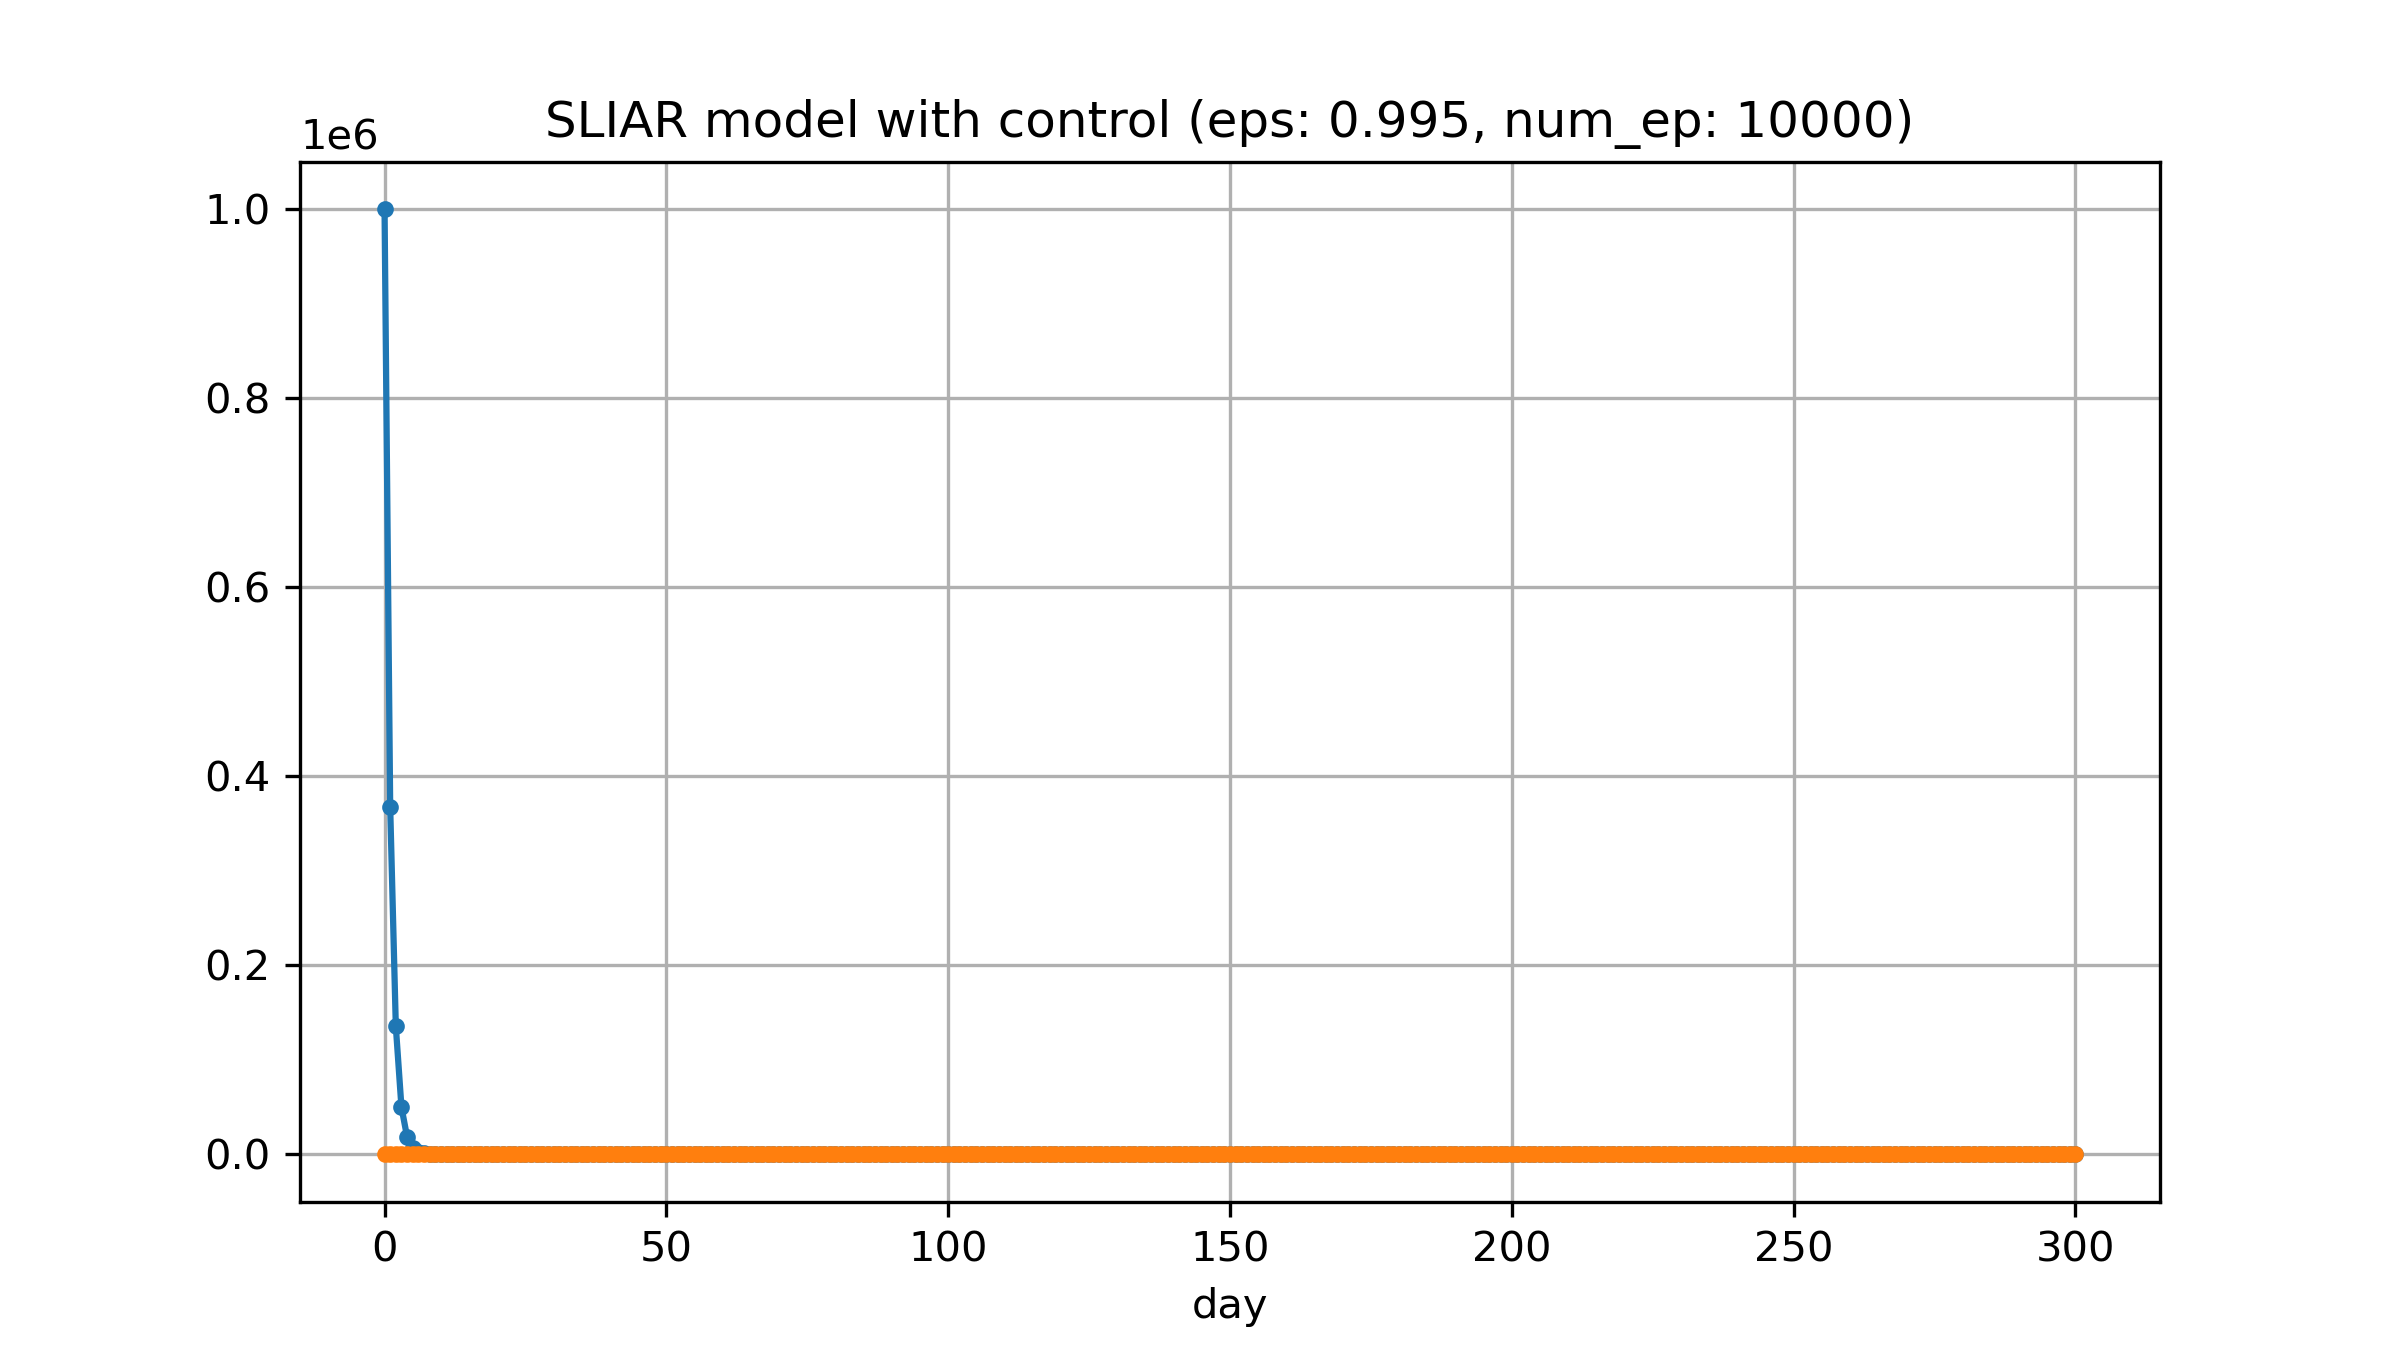
\includegraphics[width=0.48\textwidth]{../발표 자료/SLIAR_w_control_0.995,10000.png}
        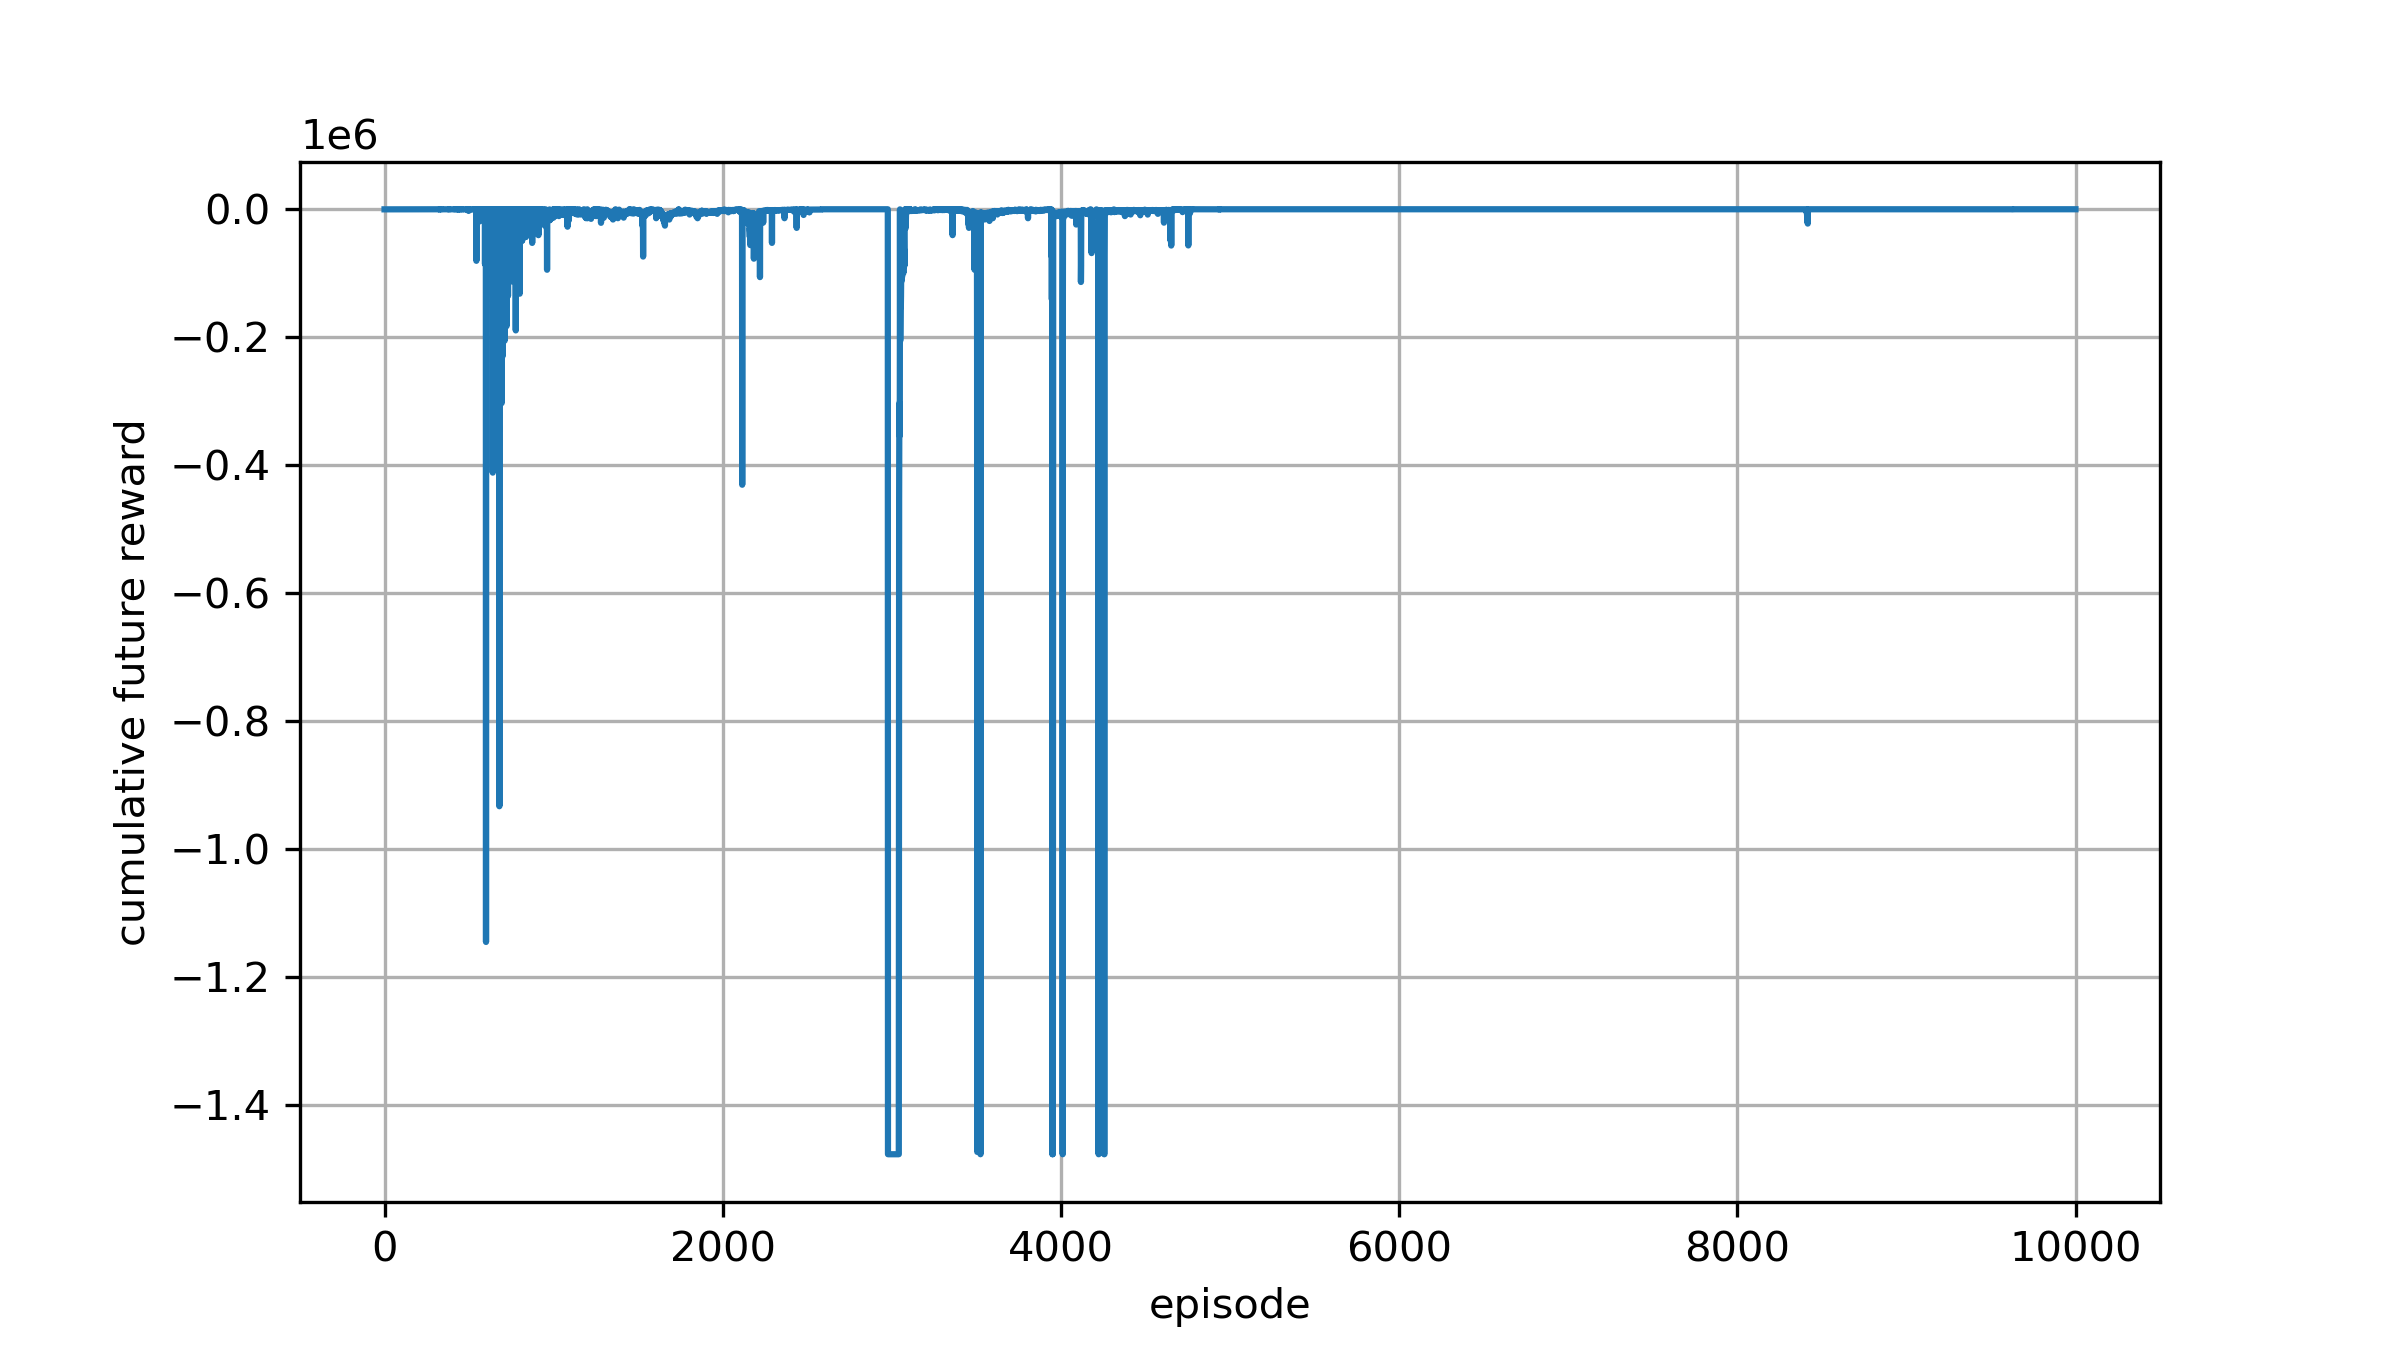
\includegraphics[width=0.48\textwidth]{../발표 자료/SLIAR_score_0.995,10000.png}
    \end{wrapfigure}

    {\fontsize{15}{50} \selectfont Initial}
    % {\fontsize{size}{baselineskip} \selectfont content}
    \hfill \break
    \hfill \break

    \; max time: 300
    \hfill \break

    \; epsilon start: 1
    \hfill \break

    \; epsilon decay: 0.995

    % \, 한 칸
    % \; 두 칸
    % \quad 네 칸
    % \qquad 여덟 칸

\end{frame}


% new page

\foreach \n in {1000, 2000, 4000, 8000, 16000} {
    \begin{frame}{Case 1\_ Learning result}
        
        After \texttt{\n} episodes learning,

        \begin{figure}[tb]
            \includegraphics[height=0.45\textheight]{../발표 자료/\n result.png}
        \end{figure}
    \end{frame}
}

\end{document}
